\documentclass[main.tex]{subfiles}

\begin{document}

  \section{Intersections}\label{sec:intersections}

  Recall, that in \S \ref{m-subsec:cycles_homo} we constructed an explicit set of generators for $\homo$ (see Theorem
  \ref{thm:gen_set}), namely
  \begin{equation}
    \Gamma = \left\{  \gamma_{e}^{(l)}  \mid  0 \le l < m-1,  e \in E  \right\}.
  \end{equation}
  Here, we show how compute the intersection pairing on $\Gamma$. The corresponding intersection matrix is composed of
  $(n-1)^2$ blocks of dimension $m-1$:
  \begin{equation}
   K_{\Gamma} = \left( K_{i,j} \right)_{1\le i,j \le n-1}
  \end{equation}
  where $i,j$ correspond to edges $e_i,e_j$ in the spanning tree $T = (X,E)$ and
  \begin{equation}
    K_{i,j} = \left(\gamma_{e_i}^{(k)} \circ \gamma_{e_j}^{(l)} \right)_{0 \le k,l < m-1}.
  \end{equation}
  Thus, $K_{\Gamma}$ can be explicitly determined by the formulas in Theorem \ref{m-thm:intsec_numb} which is stated below.
  The rest of this section is concerned with its proof.

  Very importantly, for edges $(a,b),(c,d) \in E$, by construction of the spanning tree, we can restrict to intersections $\left(\cyab^{(k)} \circ \cycd^{(l)}\right)$ 
  such that $c$ is either $a$ or $b$.

   \begin{thm}[Intersection numbers]\label{thm:intsec_numb}
      Let $(a,b),(c,d) \in E$. The intersections of the corresponding cycles $\cyabk, \cycdl \in \Gamma$ are given by
      \begin{equation}
          \left(\cyab^{(k)} \circ \cycd^{(l)}\right)
          = \begin{cases}
              1  &\text{ if } l-k \equiv s_+ \bmod m,\\
              -1 &\text{ if } l-k \equiv s_- \bmod m,\\
              0 &\text{ otherwise,}
          \end{cases}
      \end{equation}
      where $s_+$, $s_-$ are given by the following table, which covers all
      cases occurring in the algorithm
      \begin{center}
      \begin{tabular}{cccc}
          \toprule
          & Case & $s_+$ & $s_-$ \\
          \midrule
         (i) & $a=c$ and $b=d$ & $1$ & $-1$ \\
         (ii) & $b=c$ & $-s_b$ & $1-s_b$ \\
         (iii) & $a=c$ and $\rho>0$ & $1-s_a$ & $-s_a$ \\
         (iv) & $a=c$ and $\rho<0$ & $-s_a$ & $-1-s_a$\\
         (v) & $\set{a,b}\cap\set{c,d}=\varnothing$ & \multicolumn{2}{c}{no intersection} \\
          \bottomrule
      \end{tabular}
      \end{center}
      and where $s_x \in \Z$ for $x\in\set{a,b}$ is given by
      \begin{equation}\label{eq:s_x}
	    s_x := \frac{1}{2\pi}\left( \rho + m \cdot \arg \left( \frac{C_{c,d} \ytcd(x)}{C_{a,b}\ytab(x)} \right) 
	    \right)
      \end{equation}
     and
      \begin{equation}
          \rho = \arg \left( \frac{b-a}{d-c} \right) + \delta_{b=c}\pi
      \end{equation}
 \end{thm}
 
 \bigskip
 The proof of Theorem is contained in the following exposition. \\ 
  Consider
  two cycles $\cyab^{(k)},\cycd^{(l)} \in \Gamma$ and
  recall from \S \ref{m-subsec:roots_branches} their definition 
   \begin{align}\label{eq:def_cyabk}
      \cyabk & = \{  (x,\zeta^k \yab(x))  \mid  x \in [a,b]  \} \cup \{  (x,\zeta^{k+1} \yab(x))  \mid  x \in [b,a]  \}, \\
      \cycdl & = \{  (x,\zeta^l \ycd(x))  \mid  x \in [c,d]  \} \cup \{  (x,\zeta^{l+1} \ycd(x))  \mid  x \in [c,d]  \},
   \end{align}
  where $\zeta^k\yab(x),\zeta^l\ycd(x)$ are branches of $\cu$ that are analytic on open sets $\vab$ and $\vcd$ 
  (see Figure \ref{m-fig:set_vab}) respectively.
  \begin{proof}\let\qed\relax (of case $(v)$) \\
  We immediately see that that these cycles cannot have a common point, if $[a,b] \cap [c,d] = \varnothing$. Since
  $(a,b),(c,d)$ are edges in a spanning tree this is equivalent to $\{a,b\} \cap \{c,d\} = \varnothing$, thus
  proving $(v)$.
  \end{proof}
   In order to prove $(i)-(iv)$ we have to introduce some machinery. Since the $\yab(x),\ycd(x)$ are branches of $\cu$,
   on the set $\C \setminus X$
   we can define the \emph{shifting function}
   $s(x)$, that takes values in $\Z/m\Z$, implicitly via
  \begin{equation}\label{eq:shift_func}
   \zeta^{s(x)} = \frac{\ycd(x)}{\yab(x)}.
   \end{equation}
  Naturally, \eqref{eq:shift_func} extends to the other analytic branches via
  \begin{equation}
   \zeta^{s(x)+l-k} = \frac{\zeta^l\ycd(x)}{\zeta^k\yab(x)}.
   \end{equation}
   We can now introduce the set $V = \vab \cap \vcd$. If $\{a,b\} \cap \{c,d\} \ne \varnothing$, then $V$ is non-empty
  and it has the property that the shifting function $s(x)$ is well-defined on $V$ and, since $\yab(x)$ and $\ycd(x)$ are 
  both analytic on $V$, constant on its 
  connected components.
  
  In \S \ref{m-subsec:riemann_surface} we established that multiplication of a branch with $\zeta$ corresponds to moving
  one sheet up on the Riemann surface.
  We can interpret the value of the shifting function geometrically as
  $\cycdl$ running $s(\xt)+l-k$ sheets above $\cyabk$ at a point $\xt \in V$.
  
 This information can be used to determine the intersection number in the following way. We deform the cycles homotopically
 such that $\pr(\cyabk) \cap \pr(\cycdl) = \{ \xt \}$ for some $\xt \in V$. Consequently, on $\cu$ they can at most intersect in
 points in $\pr^{-1}(\xt)$. By definition, any cycle in $\Gamma$ only runs on two neighbouring sheets, which already implies
 \begin{equation}
   \left(\cyab^{(k)} \circ \cycd^{(l)}\right) = 0, \quad \text{if} \quad  s(\xt)+l-k \not\in \{-1,0,1\}.
 \end{equation}
  In the other cases we can determine the
  sign of possible intersections by taking into account the orientation of the cycles.
  
 We continue the proof with the next simplest case:
 \begin{proof}\let\qed\relax (of case $(i)$) \\
 Here we have $[a,b] = [c,d]$. We deform the cycles such that they only intersect above
 $\xt = \frac{b+a}{2} \in  \vab= V$.
 We easily see that $s(\xt) + l - k = l - k$ and that trivially $\left( \cyabk \circ \cyabk \right) = 0$ holds. The remaining cases,
 where $l = k \pm 1$, are handled in Figure \ref{m-fig:int_self_shift} below.
   Illustrated are the cycles $\cyabk$ (black),
      $\cyab^{(k+1)}$ (red) and $\cyab^{(k-1)}$ (green).
    \begin{figure}[H]
      \begin{center}
   \begin{tikzpicture}
% Intersections self-shifts
% Sheet 4
     \draw [densely dashed] (-3,3) -- (-1.8,3); 
     \draw [densely dashed] (3,3) -- (1.8,3); 
     \draw (-1.8,3) circle (1.3pt); 
     \draw (1.8,3) circle (1.3pt);
     \draw [red] (-2.5,3) .. controls (-2.5,2.6) and (-1,2.4) .. (0,3) [halfarrow2];
     \draw [red] (0,3) .. controls (1,3.6) and (2.5,3.4) .. (2.5,3) [halfarrow2];


% Sheet 3
     \draw [densely dashed] (-3,1) -- (-1.8,1); 
     \draw [densely dashed] (3,1) -- (1.8,1); 
     \draw (-1.8,1) circle (1.3pt); 
     \draw (1.8,1) circle (1.3pt);
     \draw[red] (-2.5,1) .. controls (-2.5,1.6) and (-1,1.4) .. (0,1) [halfarrow1];
     \draw[red] (0,1) .. controls (1,0.6) and (2.5,0.4) .. (2.5,1) [halfarrow1];
     \draw (-2.5,1) .. controls (-2.5,0.6) and (-1,0.4) .. (0,1) [halfarrow2];
     \draw (0,1) .. controls (1,1.6) and (2.5,1.4) .. (2.5,1) [halfarrow2];

% Intersections
    \draw (0,1) node[cross=3pt,black]{};
    \draw (0,1.3) node {$+1$};
    \draw (-1.8,0) node {$a$};  
    \draw (0,0) node {$\pr^{-1}\{\xt\}$}; 
    \draw (1.8,0) node {$b$};

% Sheet 2
    \draw [densely dashed] (-3,-1) -- (-1.8,-1); 
    \draw [densely dashed] (3,-1) -- (1.8,-1); 
    \draw (-1.8,-1) circle (1.3pt); 
    \draw (1.8,-1) circle (1.3pt);
    \draw (-2.5,-1) .. controls (-2.5,-0.4) and (-1,-0.6) .. (0,-1) [halfarrow1];
    \draw (0,-1) .. controls (1,-1.4) and (2.5,-1.6) .. (2.5,-1) [halfarrow1];
    \draw [green] (-2.5,-1) .. controls (-2.5,-1.4) and (-1,-1.6) .. (0,-1) [halfarrow2];
    \draw [green] (0,-1) .. controls (1,-0.4) and (2.5,-0.6) .. (2.5,-1) [halfarrow2];

% Intersection
    \draw (0,-1) node[cross=3pt,black]{};
    \draw (0,-1.3) node {$-1$};

% Sheet 1
    \draw [densely dashed] (-3,-3) -- (-1.8,-3); 
    \draw [densely dashed] (3,-3) -- (1.8,-3); 
    \draw (-1.8,-3) circle (1.3pt); 
    \draw (1.8,-3) circle (1.3pt);
    \draw[green] (-2.5,-3) .. controls (-2.5,-2.4) and (-1,-2.6) .. (0,-3) [halfarrow1];
    \draw[green] (0,-3) .. controls (1,-3.4) and (2.5,-3.6) .. (2.5,-3) [halfarrow1];
\end{tikzpicture}
      \end{center}
    \caption{Intersections of self-shifts.}
    \label{fig:int_self_shift}
\end{figure}
  We see that independently of $s(\xt)$, $s_+ = (k+1)-k = 1$ and $s_- = (k-1)-k = -1$ are as claimed.
 \end{proof}

  For $(ii)-(iv)$ we have that $[a,b] \cap [c,d] = \{ x_0 \}$, where $x_0$ is either $a$ or $b$. Unfortunately, in these cases $s(x_0)$ is not
  well-defined.
  
 Following our strategy, we choose a point $\xt \in \C \setminus X$ on the bisectrix of
  $[a,b]$ and $[c,d]$ that is close enough to $x_0$ such that $[\xt,x_0[ \subset V = \vab \cap \vcd$
  (see Figure \ref{m-fig:set_v_both} below).
  
  Then we can easily compute $s(\xt)$ using the argument function
  \begin{equation}\label{eq:sxt}
   s(\xt) = \frac{m}{2\pi} \arg \left( \frac{\ycd(\xt)}{\yab(\xt)} \right).
  \end{equation}
  
    \begin{figure}[H]
      \begin{center}
   \scalebox{.9}{\begin{tikzpicture}
% Set V for b=c and a=c
    
  \draw (-3.3,0) node {$a$};  \draw (-0.3,0) node {$b$}; \draw (-1.8,0) node {$V_{a,b}$};
  \draw (-3.6,0) circle (0.8pt); 
  \draw  (0,0) circle (0.8pt);
  \draw [densely dashed] (-4.8,0) -- (-3.6,0);   
  \draw [densely dashed] (1.5,0) -- (0,0);
  \draw (-4.2,0.05) .. controls (-3.8,1.5) and (0.2,1.5) .. (0.6,0.05);
  \draw (-4.2,-0.05) .. controls (-3.8,-1.5) and (0.2,-1.5) .. (0.6,-0.05);
  \draw (-4.2,-0.05) -- (-3.5,-0.05); \draw (0.6,-0.05) -- (-0.1,-0.05);
  \draw (-4.2,0.05) -- (-3.5,0.05); \draw (0.6,0.05) -- (-0.1,0.05);
  \draw (-3.5,0.05) -- (-3.5,-0.05); \draw (-0.1,0.05) -- (-0.1,-0.05);
    
  \draw (1.8,3.117) circle (0.8pt); 
  \draw (1.8,2.8) node {$d$}; \draw (1.0,1.5) node {$V_{b,d}$};
  \draw [densely dashed] (1.8,3.117) -- (2.4,4.156); 
  \draw [densely dashed] (0,0) -- (-0.8,-1.386);
  \draw [rotate=240,shift={(0,0)}] (-4.2,0.05) .. controls (-3.8,1.5) and (0.2,1.5) .. (0.6,0.05);
  \draw [rotate=240,shift={(0,0)}] (-4.2,-0.05) .. controls (-3.8,-1.5) and (0.2,-1.5) .. (0.6,-0.05);
  \draw [rotate=240,shift={(0,0)}] (-4.2,-0.05) -- (-3.5,-0.05);  \draw [rotate=240,shift={(0,0)}] (0.6,-0.05) -- (-0.1,-0.05);
  \draw [rotate=240,shift={(0,0)}](-4.2,0.05) -- (-3.5,0.05); \draw [rotate=240,shift={(0,0)}] (0.6,0.05) -- (-0.1,0.05);
  \draw [rotate=240,shift={(0,0)}] (-3.5,0.05) -- (-3.5,-0.05); \draw [rotate=240,shift={(0,0)}] (-0.1,0.05) -- (-0.1,-0.05);
       
  \draw [dotted] (-1,1.732) -- (0.75,-1.3);
  \draw (-0.35,0.606) circle (0.8pt); \draw (-0.1,0.6) node {$\tilde{x}$};

  
  % Set V = V_ab \cap V_ad

  \draw (5.1,0.3) node {$a$};
  \draw (7.3,2.3) node {$b$};
  \draw (7.3,-2.3) node {$d$};
  \draw (6.5,1.5) node {$V_{a,b}$};
  \draw (6.5,-1.5) node {$V_{a,d}$};
  %\draw (-1.8,0) node {$V_{a,b}$};
  \draw (5,0) circle (0.8pt);
  \draw (7.545,-2.545) circle (0.8pt); 
  \draw (7.545,2.545) circle (0.8pt);
  \draw [densely dashed] (5,0) -- (5-0.848,0.848);   
  \draw [densely dashed] (5,0) -- (5-0.848,-0.848);
  \draw [densely dashed] (7.545,-2.545) -- (8.39,-3.39);
  \draw [densely dashed] (7.545,2.545) -- (8.39,3.39);
  \draw [dotted] (5-1,0) -- (8,0);
  \draw (5.5,0) circle (0.8pt); \draw (5.7,0) node {$\tilde{x}$};
  
  \draw [shift={(5,0)},rotate=225] (0.6,0.05) .. controls (0.2,1.5) and (-3.8,1.5) .. (-4.2,0.05);
  \draw [shift={(5,0)},rotate=225] (0.6,-0.05) .. controls  (0.2,-1.5) and (-3.8,-1.5) .. (-4.2,-0.05);
  \draw [shift={(5,0)},rotate=225] (-3.5,-0.05) -- (-4.2,-0.05); \draw [shift={(5,0)},rotate=225] (-0.1,-0.05) -- (0.6,-0.05);
  \draw [shift={(5,0)},rotate=225] (-3.5,0.05) -- (-4.2,0.05); \draw [shift={(5,0)},rotate=225] (-0.1,0.05) -- (0.6,0.05);
  \draw [shift={(5,0)},rotate=225] (-3.5,-0.05) -- (-3.5,0.05);  \draw [shift={(5,0)},rotate=225] (-0.1,-0.05) -- (-0.1,0.05);
  
  \draw [shift={(5,0)},rotate=-225] (0.6,0.05) .. controls (0.2,1.5) and (-3.8,1.5) .. (-4.2,0.05);
  \draw [shift={(5,0)},rotate=-225] (0.6,-0.05) .. controls  (0.2,-1.5) and (-3.8,-1.5) .. (-4.2,-0.05);
  \draw [shift={(5,0)},rotate=-225] (-3.5,-0.05) -- (-4.2,-0.05); \draw [shift={(5,0)},rotate=-225] (-0.1,-0.05) -- (0.6,-0.05);
  \draw [shift={(5,0)},rotate=-225] (-3.5,0.05) -- (-4.2,0.05); \draw [shift={(5,0)},rotate=-225] (-0.1,0.05) -- (0.6,0.05);
  \draw [shift={(5,0)},rotate=-225] (-3.5,-0.05) -- (-3.5,0.05);  \draw [shift={(5,0)},rotate=-225] (-0.1,-0.05) -- (-0.1,0.05);
\end{tikzpicture}
}
      \end{center}
     \vspace{-1cm}
    \caption{The set $V = \vab \cap \vcd$ for $b=c$ (left) and $a=c$ (right).}
    \label{fig:set_v_b=c}
\end{figure}
   
   
   
   
   
   \begin{proof}\let\qed\relax (of case $(ii)$) \\
   In this case ($x_0 = b = c$) we choose $\xt$ on the upper bisectrix, as shown in Figure \ref{m-fig:set_v_both}, 
   and compute $s(\xt)$ with \eqref{m-eq:sxt}.
   
   Again, the non-trivial cases where $s(\xt) + l - k \in \{1,0,-1\}$, are shown in Figure \ref{m-fig:int_b=c}.
   Illustrated are the cycles $\cyab^k$ (black), $\cycd^{k-s(\xt)}$ (gray), $\cycd^{k-s(\xt) + 1 }$ (green) and
    $\cycd^{k-s(\xt)-1}$ (red),
    \begin{figure}[H]
      \begin{center}
   \begin{tikzpicture}
% Intersections for b = c

  \draw (-3.6,2) node {$a$};  \draw (0,2) node {$b$};  \draw (1.8,5.117) node {$d$}; 
  
  
% Intersections
    \draw (-0.35,4.606) node[cross=3pt,black,rotate=80]{};
    \draw (-0.25,5) node {$-1$};    
    \draw (-0.35,0.606) node[cross=3pt,black,rotate=80]{};
    \draw (0.0,0.5) node {$+1$}; 

% Sheet 4
    \draw (-3.6,8) circle (0.8pt); 
    \draw (0,8) circle (0.8pt);   
    \draw (1.8,11.117) circle (0.8pt); 
    \draw [densely dashed] (-4.8,8) -- (-3.6,8);
    \draw [densely dashed] (0,8) -- (1.2,8); 
    \draw [densely dashed] (0,8) -- (-0.6,8-1.04);
    \draw [densely dashed] (1.8,11.117) -- (2.4,12.156);
    \draw [green] (1.95,11.377) .. controls (0.2,12) and (1.5,6.8) .. (-0.4,7.3) [halfarrow1];

% Sheet 3
    \draw (-3.6,4) circle (0.8pt); 
    \draw (0,4) circle (0.8pt);   
    \draw (1.8,7.117) circle (0.8pt);   
    \draw [densely dashed] (-4.8,4) -- (-3.6,4);
    \draw [densely dashed] (0,4) -- (1.2,4); 
    \draw [densely dashed] (0,4) -- (-0.6,4-1.04);
    \draw [densely dashed] (1.8,7.117) -- (2.4,8.156);
    \draw (-4.1,4) .. controls (-4,2.5) and (0.4,5.95) .. (0.45,4) [halfarrow2];
    \draw [green] (1.95,7.377) .. controls (2.8,7) and (2,5.5) .. (-0.35,4.606) [halfarrow2];
    \draw [green] (-0.35,4.606) arc(110:245:0.7cm) [halfarrow2];
    \draw [gray] (1.95,7.377) .. controls (0.2,8) and (1.5,2.8) .. (-0.4,3.3) [halfarrow1];
  
  
% Sheet 2
    \draw (-3.6,0) circle (0.8pt); 
    \draw (0,0) circle (0.8pt);   
    \draw (1.8,3.117) circle (0.8pt); 
    \draw [densely dashed] (-4.8,0) -- (-3.6,0);
    \draw [densely dashed] (0,0) -- (1.2,0); 
    \draw [densely dashed] (0,0) -- (-0.6,-1.04);
    \draw [densely dashed] (1.8,3.117) -- (2.4,4.156);
    \draw (-4.1,0) .. controls (-4,1) and (0.4,1.5) .. (-0.45,0.4) [halfarrow1];
    \draw [gray] (1.95,3.377) .. controls (2.8,3) and (2,1.5) .. (-0.35,0.606) [halfarrow2];
    \draw (-0.45,0.4) arc(150:342:0.5cm) [halfarrow1];
    \draw [gray] (-0.35,0.606) arc(110:245:0.7cm) [halfarrow2];
    \draw [red] (1.95,3.377) .. controls (0.2,4) and (1.5,-1.2) .. (-0.4,-0.7) [halfarrow1];


% Sheet 1
    \draw [black] (-3.6,-4) circle (0.8pt); 
    \draw [black] (0,-4) circle (0.8pt);   
    \draw [black] (1.8,-0.883) circle (0.8pt); 
    \draw [densely dashed] (-4.8,-4) -- (-3.6,-4);
    \draw [densely dashed] (0,-4) -- (1.2,-4); 
    \draw [densely dashed] (0,-4) -- (-0.6,-5.04);
    \draw [densely dashed] (1.8,-4+3.117) -- (2.4,0.156);
    \draw [red] (-0.35,-3.394) arc(110:245:0.7cm) [halfarrow2];
    \draw [red] (1.95,-0.623) .. controls (2.8,-1) and (2,-2.5) .. (-0.35,-3.394) [halfarrow2];
 
\end{tikzpicture}
      \end{center}
    \caption{Intersections for $b=c$.}
    \label{fig:int_b=c}
   \end{figure}
    By Lemma \ref{lemma:sxt=sx} (1) we have $s(\xt) = s_b$, which implies
    \begin{align*}
    & s_+ = k-s(\xt)-k = s_b, \\
    & s_- = k-s(\xt)+1-k = 1-s_b
    \end{align*}
  as claimed.
  \end{proof}
 
%  \begin{figure}[H]
%       \begin{center}
%    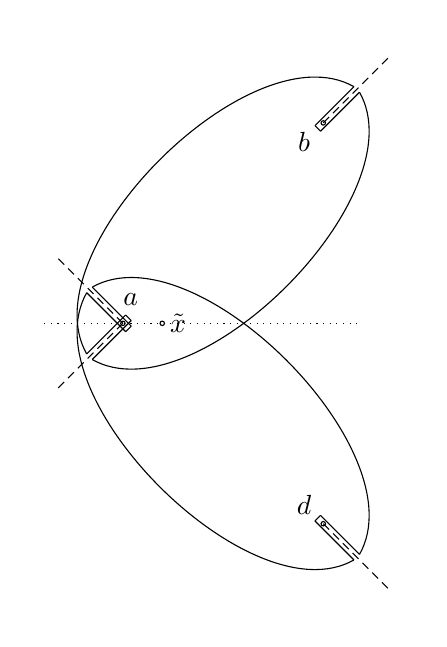
\begin{tikzpicture}
% Set V = V_ab \cap V_ad

  \draw (0.1,0.3) node {$a$};
  \draw (2.3,2.3) node {$b$};
  \draw (2.3,-2.3) node {$d$};
  \draw (1.5,1.5) node {$\vab$};
  \draw (1.5,-1.5) node {$\vbd$};
  %\draw (-1.8,0) node {$V_{a,b}$};
  \draw (0,0) circle (0.8pt);
  \draw (2.545,-2.545) circle (0.8pt); 
  \draw (2.545,2.545) circle (0.8pt);
  \draw [densely dashed] (0,0) -- (-0.848,0.848);   
  \draw [densely dashed] (0,0) -- (-0.848,-0.848);
  \draw [densely dashed] (2.545,-2.545) -- (3.39,-3.39);
  \draw [densely dashed] (2.545,2.545) -- (3.39,3.39);
  \draw [dotted] (-1,0) -- (3,0);
  \draw (0.5,0) circle (0.8pt); \draw (0.7,0) node {$\tilde{x}$};
  
  \draw [rotate=225] (0.6,0.05) .. controls (0.2,1.5) and (-3.8,1.5) .. (-4.2,0.05);
  \draw [rotate=225] (0.6,-0.05) .. controls  (0.2,-1.5) and (-3.8,-1.5) .. (-4.2,-0.05);
  \draw [rotate=225] (-3.5,-0.05) -- (-4.2,-0.05); \draw [rotate=225] (-0.1,-0.05) -- (0.6,-0.05);
  \draw [rotate=225] (-3.5,0.05) -- (-4.2,0.05); \draw [rotate=225] (-0.1,0.05) -- (0.6,0.05);
  \draw [rotate=225] (-3.5,-0.05) -- (-3.5,0.05);  \draw [rotate=225] (-0.1,-0.05) -- (-0.1,0.05);
  
  \draw [rotate=-225] (0.6,0.05) .. controls (0.2,1.5) and (-3.8,1.5) .. (-4.2,0.05);
  \draw [rotate=-225] (0.6,-0.05) .. controls  (0.2,-1.5) and (-3.8,-1.5) .. (-4.2,-0.05);
  \draw [rotate=-225] (-3.5,-0.05) -- (-4.2,-0.05); \draw [rotate=-225] (-0.1,-0.05) -- (0.6,-0.05);
  \draw [rotate=-225] (-3.5,0.05) -- (-4.2,0.05); \draw [rotate=-225] (-0.1,0.05) -- (0.6,0.05);
  \draw [rotate=-225] (-3.5,-0.05) -- (-3.5,0.05);  \draw [rotate=-225] (-0.1,-0.05) -- (-0.1,0.05);

\end{tikzpicture}

%       \end{center}
%     \caption{The set $V = \vab \cap \vad$.}
%     \label{fig:set_v_a=c}
% \end{figure}
   
 
 
 \begin{proof}(of cases $(iii) + (iv)$)
 In this case ($x_0 = b = c$) we choose $\xt$ on the inner bisectrix, as shown in Figure \ref{m-fig:set_v_a=c}, 
   and compute $s(\xt)$ with \eqref{m-eq:sxt}.
 \end{proof}

  \begin{figure}[H]
      \begin{center}
   \scalebox{0.9}{\begin{tikzpicture}

% Variables
%\draw (-4.5,3) node{$b$};
%\draw (-1,0) node{$a$};
%\draw (-4.5,-3) node{$d$};



% Intersections
    \draw (5.5,0) node[cross=3pt,black,rotate=60]{};
    \draw (5.6,0.4) node {$-1$};    
    \draw (10.5,0) node[cross=3pt,black,rotate=60]{};
    \draw (11,0) node {$+1$};
 
% Sheet 1
\draw (0,0) circle (0.8pt);
\draw (2.545,-2.545) circle (0.8pt); 
\draw (2.545,2.545) circle (0.8pt);
\draw [densely dashed] (0,0) -- (-0.848,0.848);   
\draw [densely dashed] (0,0) -- (-0.848,-0.848);
\draw [densely dashed] (2.545,-2.545) -- (3.39,-3.39);
\draw [densely dashed] (2.545,2.545) -- (3.39,3.39);    

\draw [red]  (-0.353,0.353) .. controls (0.8,1.3) and (1.3,-3.7) .. (2.757,-2.757) [halfarrow1];


% Sheet 2
\draw (5,0) circle (0.8pt);
\draw (7.545,-2.545) circle (0.8pt); 
\draw (7.545,2.545) circle (0.8pt);
\draw [densely dashed] (5,0) -- (5-0.848,0.848);   
\draw [densely dashed] (5,0) -- (5-0.848,-0.848);
\draw [densely dashed] (7.545,-2.545) -- (8.39,-3.39);
\draw [densely dashed] (7.545,2.545) -- (8.39,3.39); 

\draw [black] (5.5,0) arc (30:200:0.5cm) [halfarrow2];
\draw [black] (5.5,0) .. controls (6.25,-0.75) and (8.6,2.5) .. (7.757,2.757) [halfarrow1];

\draw [red]  (5-0.353,0.353) .. controls (2.9,-1.1) and (9.1,-1.6) .. (7.757,-2.757) [halfarrow2];
\draw [gray]  (5-0.353,0.353) .. controls (5.8,1.3) and (6.3,-3.7) .. (7.757,-2.757) [halfarrow1];


% Sheet 3
\draw (10,0) circle (0.8pt);
\draw (12.545,-2.545) circle (0.8pt); 
\draw (12.545,2.545) circle (0.8pt);
\draw [densely dashed] (10,0) -- (10-0.848,0.848);   
\draw [densely dashed] (10,0) -- (10-0.848,-0.848);
\draw [densely dashed] (12.545,-2.545) -- (13.39,-3.39);
\draw [densely dashed] (12.545,2.545) -- (13.39,3.39);

\draw [black] (10-0.353,-0.353) .. controls (10.8,-1.3) and (11.3,3.7) .. (12.757,2.757) [halfarrow2]; 
\draw [green]  (10-0.353,0.353) .. controls (10.8,1.3) and (11.3,-3.7) .. (12.757,-2.757) [halfarrow1];
\draw [gray]  (10-0.353,0.353) .. controls (7.9,-1.1) and (14.1,-1.6) .. (12.757,-2.757) [halfarrow2];


% Sheet 4
\draw (15,0) circle (0.8pt);
\draw (17.545,-2.545) circle (0.8pt); 
\draw (17.545,2.545) circle (0.8pt);
\draw [densely dashed] (15,0) -- (15-0.848,0.848);   
\draw [densely dashed] (15,0) -- (15-0.848,-0.848);
\draw [densely dashed] (17.545,-2.545) -- (18.39,-3.39);
\draw [densely dashed] (17.545,2.545) -- (18.39,3.39);

\draw [green]  (15-0.353,0.353) .. controls (12.9,-1.1) and (19.1,-1.6) .. (17.757,-2.757) [halfarrow2];


% Branch points
\draw (15.5,0) node {$a$};
\draw (17,2.545) node {$b$};
\draw (17,-2.545) node {$d$};
\end{tikzpicture}}
      \end{center}
    \caption{Intersections for $a=c$.}
    \label{fig:int_b=c}
   \end{figure}
 
 
  
\begin{lemma}\label{lemma:sxt=sx}
  \begin{itemize}
   \item[(1)] In the proof of case $(ii)$ of Theorem \ref{m-thm:intsec_numb}, choosing $\xt$ on the upper bisectrix
   of $[a,b],[b,d]$, suffices $s(\xt) = s_b$ as defined in \eqref{m-eq:sxt} and \eqref{m-eq:s_x} respectively.
    \item[(2)] In the proof of the cases $(iii)$ and $(iv)$ of Theorem \ref{m-thm:intsec_numb}, choosing $\xt$ on the upper bisectrix
   of $[a,b],[a,d]$, suffices $s(\xt) = s_a$ as defined in \eqref{m-eq:sxt} and \eqref{m-eq:s_x} respectively.
  \end{itemize}
\end{lemma}
 \begin{proof}
 \todo Rework.
  With $\rho = \arg\left(\frac{b-a}{d-b}\right)$ we have that
  \begin{align*}
   & \arg (1+\ubd(x)) = \frac{\pi+\rho}{2} \quad \text{for all}  x \in [\xt,x_0[,\\
   & \arg (1-\uab(x)) = -\frac{\pi+\rho}{2} \quad \text{for all}  x \in [\xt,x_0[,\\
   & \arg (1-\ubd(x_0)) = 0,\\
   & \arg (1+\uab(x_0))= 0,
  \end{align*}
  and therefore
  \begin{align*}
   \theta = \frac{\pi+\rho}{2} - \left(-\frac{\pi+\rho}{2}\right) = \pi + \rho.
  \end{align*}
  \begin{equation}
   \equiv \frac{1}{2\pi}\left( \theta(x) + m \arg \left( \frac{ \ccd \ytcd(x)}{ \cab
   \ytab(x)} \right) \right) \bmod m
   \theta(x) = \arg(1+\ucd(x)) + \arg(1-\ucd(x)) - \arg(1+\uab(x)) - \arg(1-\ucd(x)).
  \end{equation}
    \begin{align}\label{eq:s(x)2}
  \begin{split}
   \zeta^{s(x)} & = \frac{\ycd(x)}{\yab(x)} = \frac{(1- \ucd(x)^2)\mr \ccd \ytcd(x) }{(1-\uab(x)^2)\mr \cab \ytab(x)} \\
   \Rightarrow  s(x) & \equiv \frac{m}{2\pi} \left( \arg \left( \frac{(1- \ucd(x)^2)\mr}{(1-\uab(x)^2)\mr} \right) + \arg \left( \frac{ \ccd \ytcd(x)}{ \cab
   \ytab(x)} \right) \right) \bmod m
  \end{split}
  \end{align}
 \end{proof}


\begin{rmk}
  \todo Rework. Note that depending on our choice of $\xt$ (either on the upper or the lower bisectrix), the path
  $[\xt,x_0[$ will be contained in different connected components of $V$. Although the value of
  $s(\xt)$ will change, the intersection number is independent of that choice.
\end{rmk}


%  The problem here is that $\theta(x_0)$ is not defined. We resolve this by
%   choosing a point $\xt$ on the bisectrix of
%   $[a,b]$ and $[c,d]$, close enough to $x_0$, such that $[\xt,x_0[ \subset  V = \vab \cap \vab$. 
%   Staying away from the branch cuts (see Figure \ref{m-fig:set_v}), $\theta(x)$ is continuous on $[\xt,x_0[$ and can be continously continued to $x_0$ (this is done below). 
%   Therefore, the limit
%   \begin{equation}
%      \theta(x_0) := \lim_{\xt \rightarrow x_0} \theta(\xt) 
%   \end{equation}
%   exists and we can compute the shifting function $s(x_0)$.

%   Assuming that the shifting number $s=s(\cyab,\cycd,\xt)$ is computed as above, we can now determine the intersections graphically. \abstandl
%   As before, the only interesting cases
%   are $s \in \{0,\pm 1\}$. Figure \ref{m-fig:int_b=c} displays the cycles $\cyab$ (black) and $\cycd$ in green ($s=1$), gray ($s=0$) and red ($s=-1$).
%   We can read off the intersection numbers
%   \begin{align*}
%     \left(\cyab \circ \cycd\right) = \begin{cases}
%                                           +1, \quad & \text{if} \quad s=0,\\
%                                           -1, \quad & \text{if} \quad s=1,\\
%                                           \quad\!0, \quad & \text{otherwise}.
%                                          \end{cases}
%   \end{align*}
%   The relation \eqref{m-eq:shift_numb_rel} extends this to $\left(\cyabl \circ \cycdk\right)$ as claimed.
%   \begin{figure}[H]
%       \begin{center}
%    \begin{tikzpicture}

  \draw (-3.6,2) node {$a$};  \draw (0,2) node {$b$};  \draw (1.8,5.117) node {$d$}; 
  
  
% Intersections
    \draw (-0.35,4.606) node[cross=3pt,black,rotate=80]{};
    \draw (-0.25,5) node {$-1$};    
      \draw (-0.35,0.606) node[cross=3pt,black,rotate=60]{};
    \draw (0.0,0.5) node {$+1$}; 

% Sheet 4
  \draw (-3.6,8) circle (0.8pt); 
  \draw (0,8) circle (0.8pt);   
  \draw (1.8,11.117) circle (0.8pt); 
  \draw [densely dashed] (-4.8,8) -- (-3.6,8);
  \draw [densely dashed] (0,8) -- (1.2,8); 
  \draw [densely dashed] (0,8) -- (-0.6,8-1.04);
  \draw [densely dashed] (1.8,11.117) -- (2.4,12.156);
  \draw [green] (1.95,11.377) .. controls (0.2,12) and (1.5,6.8) .. (-0.4,7.3) [halfarrow1];
  
% Sheet 3
  \draw (-3.6,4) circle (0.8pt); 
  \draw (0,4) circle (0.8pt);   
  \draw (1.8,7.117) circle (0.8pt); 
  
  \draw [densely dashed] (-4.8,4) -- (-3.6,4);
  \draw [densely dashed] (0,4) -- (1.2,4); 
  \draw [densely dashed] (0,4) -- (-0.6,4-1.04);
  \draw [densely dashed] (1.8,7.117) -- (2.4,8.156);
  \draw (-4.1,4) .. controls (-4,2.5) and (0.4,5.95) .. (0.35,4) [halfarrow2];
  \draw [green] (1.95,7.377) .. controls (2.8,7) and (2,5.5) .. (-0.35,4.606) [halfarrow2];
  \draw [green] (-0.35,4.606) arc(110:245:0.7cm) [halfarrow2];
  \draw [gray] (1.95,7.377) .. controls (0.2,8) and (1.5,2.8) .. (-0.4,3.3) [halfarrow1];
 
 
% Sheet 2
\draw (-3.6,0) circle (0.8pt); 
\draw (0,0) circle (0.8pt);   
\draw (1.8,3.117) circle (0.8pt); 

  \draw [densely dashed] (-4.8,0) -- (-3.6,0);
  \draw [densely dashed] (0,0) -- (1.2,0); 
  \draw [densely dashed] (0,0) -- (-0.6,-1.04);
  \draw [densely dashed] (1.8,3.117) -- (2.4,4.156);
    \draw (-4.1,0) .. controls (-4,1) and (0.2,1.5) .. (-0.35,0.606) [halfarrow1];
    \draw [gray] (1.95,3.377) .. controls (2.8,3) and (2,1.5) .. (-0.35,0.606) [halfarrow2];
    \draw (-0.35,0.606) arc(150:233:0.7cm) [halfarrow1];
     \draw [gray] (-0.35,0.606) arc(110:245:0.7cm) [halfarrow2];
     \draw [red] (1.95,3.377) .. controls (0.2,4) and (1.5,-1.2) .. (-0.4,-0.7) [halfarrow1];


% Sheet 1
\draw [black] (-3.6,-4) circle (0.8pt); 
\draw [black] (0,-4) circle (0.8pt);   
\draw [black] (1.8,-0.883) circle (0.8pt); 
    \draw [densely dashed] (-4.8,-4) -- (-3.6,-4);
  \draw [densely dashed] (0,-4) -- (1.2,-4); 
  \draw [densely dashed] (0,-4) -- (-0.6,-5.04);
  \draw [densely dashed] (1.8,-4+3.117) -- (2.4,0.156);
    \draw [red] (-0.35,-3.394) arc(110:245:0.7cm) [halfarrow2];
    \draw [red] (1.95,-0.623) .. controls (2.8,-1) and (2,-2.5) .. (-0.35,-3.394) [halfarrow2];
 
\end{tikzpicture}
%       \end{center}
%     \caption{Intersections for $b=c$ and $s \in \{1,0,-1\}$.}
%     \label{fig:int_b=c}
% \end{figure}

%  \begin{defn}\label{def:shift_numb}
%  Let $\cyab, \cycd \in C$ be elementary cycles and let $V = V_{a,b} \cap V_{c,d}$. Then, $\yab$ and $\ycd$ are analytic functions with no zeros on $V$. For each $x \in V$ there
%  exists an $s \in \Z/m\Z$ such that
%  \begin{align}
%    \frac{\ycd(x)}{\yab(x)} = \zeta^s .
%  \end{align}
%  We say $s  = s(\cyab,\cycd,x)$ is the \emph{shfiting number of $\cyab$ and $\cycd$ at $x$}.
%  \end{defn}
%  This definition naturally extends to shifts of elementary cycles via
%  \begin{align}
%    \frac{\zeta^k\ycd(x)}{\zeta^l\yab(x)} = \zeta^{s+k-l} \quad \imp \quad s(\cyabl,\cycdk,x) = s(\cyab,\cycd,x) + k - l.
%  \end{align}


%  Note that the set $V$ is not connected. It is split up into two disjoint open subsets by the local branch cuts. Although the shifting number is not constant on $V$, it is constant on its
%  connected components.
%
%  However, computing the shifting number for \emph{one} point $x \in V$ is sufficient to determine all the intersections $\left(  \cyabl \circ \cycdk \right)$.
%
%      We can compute the shiftung number for all elementary cycles $\cyab, \cycd \in C$:
%
%     \begin{thm}\label{thm:shift_numb}
%     Assume $[a,b] \cap [c,d] = \{x\}$. With notations as above and $\tau = \arg \left( \frac{d-c}{b-a} \right)$ we have that
%      \begin{align}\label{eq:shift_numb}
%        s(\alpha,\beta) = \frac{1}{2\pi} \left( \theta +  m \cdot \arg \left( \frac{(b-a)^{\frac{d}{m}} \ytab(x)}{(d-c)^{\frac{d}{m}} \ytcd(x)} \right) \right) \in \Z/m\Z,
%      \end{align}
%      where
%       \begin{align*}\theta = \begin{cases}
%                                -\pi+\tau, \quad \text{if} \quad \tau < 0 \quad \text{and} \quad (x = b = c \quad \text{or} \quad x = a = d),\\
%                               \quad\! \pi-\tau, \quad \text{if} \quad \tau \ge 0 \quad \text{and} \quad (x = b = c \quad \text{or} \quad x = a = d),\\
%                               \hspace{0.7cm} -\tau, \quad \text{if} \quad x = a = c \quad \text{or} \quad x = b = d,\\
%                               \hspace{1cm} 0, \quad \text{if} \quad x  \in  ]a,b[ \cap ]c,d[.
%                              \end{cases}
%      \end{align*}
%     \end{thm}
%     \begin{proof}
%      See \S \todo ref.
%     \end{proof}
%
%      Using this information, we obtain the intersection numbers graphically by using visualizations of $\alpha$ on $\beta$ running on different sheets.
%      However, if we find homologous cycles, whose projections do not intersect, their lifts to the surface cannot intersect.

%     At a common point $p$, that is no branch points, the notion of sheets makes sense and there exists an $s \in \Z/N\Z$ such that. This means that above the point $p$
%      $\beta_0$ runs $s$ sheets above $\alpha_0$. We will call $s = s(\alpha,\beta)$ the \textit{shifting number} of $\alpha$ and $\beta$ at $p$.
%     If $p$ is a branch point, we choose homologous paths whose $x$-projections intersect at a non-branch point and take a limit.



%        \begin{split}
%         (\cyabl \circ \cycdk) =
%         \begin{cases}
%             \hspace*{0.95cm} -1, \quad & \text{if} \quad s=0 \quad \text{and} \quad (x = b = c \quad \text{or} \quad x = a = d),\\
%       \hspace*{0.95cm} +1, \quad &\text{if} \quad s=-1 \quad \text{and} \quad (x = b = c \quad \text{or} \quad x = a = d),\\
%           \quad\! \sgn(\tau), \quad & \text{if} \quad s=0 \quad \text{and} \quad (x = a = c \quad \text{or} \quad x = b = d),\\
%             -\sgn(\tau), \quad & \text{if} \quad s=-\sgn(\tau) \quad \text{and} \quad (x = a = c \quad \text{or} \quad x = b = d),\\
%           \hspace*{0.95cm} +1, \quad &\text{if} \quad s=1 \quad \text{and} \quad [a,b] = [c,d],\\
%           \hspace*{0.95cm} -1, \quad &\text{if} \quad s=-1 \quad \text{and} \quad [a,b] = [c,d],\\
%          \hspace*{0.95cm}  \quad\! 0, \quad &\text{otherwise}.
%         \end{cases}
%        \end{split}
%       \end{align}

\end{document}
